\section{Probleemi uurimine}

Ehitusfüüsika mõistes ehituskonstruktsioon kujutab endast erinevate füüsikaliste oma-dustega kihtidest 
koosnevat materjali. Kihid võivad olla homogeensed s.t. ühest materjalist koosnevad (näiteks: betoon, vahtpolüstüreen) ja
mittehomogeensed s.t. mitmest materjalist koosnevad (näiteks: puitsõrestiksein, kus ühes kihis on nii soojusisolatsioon, 
kui ka teatud sammuga puitpostid). Homogeense ja mittehomogeense konstruktsiooni näited on toodud pildil \ref{fig:excel_table_sample}.

\begin{figure}[ht]
    \centering
    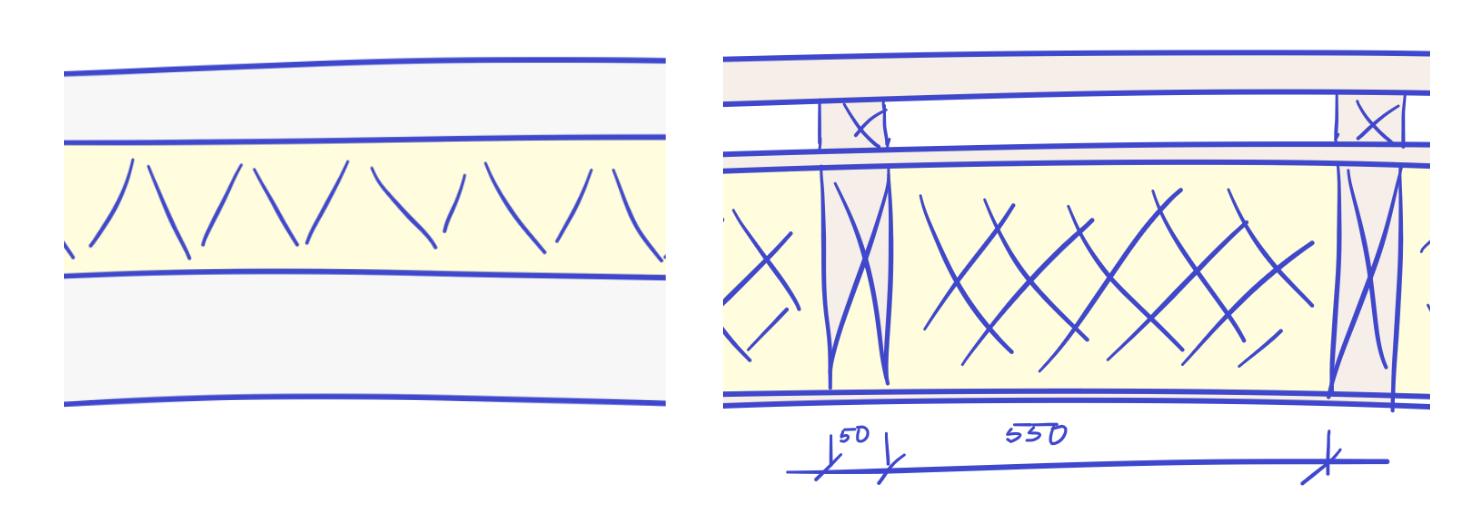
\includegraphics[width=.8\textwidth]{figures/01_analogues/06_un_non_unif_sample.png}
    \caption{\textit{Homogeense ja mittehomogeense konstruktsiooni näide}}
    \label{fig:construction_samples}
\end{figure}
\textbf{TODO: better illustration}

Ehitusfüüsika seisukohalt kõige olulisemad materjali omadused on soojuserijuhtivus \begin{math}\lambda\end{math} [W/mK]
ja veeaurutakistus, mis võib olla väljendatud mitmel viisil (neid viise on palju, aga käesolevas töös keskendutakse 
ainult järgmistele, kuna need on kõige rohkem kasutatud nii raamatutes, kui ka materjalitootjate dokumentatsioonis):
\begin{math}\mu\end{math} - diffusioonitakistustegur (materjali omadus), Sd[m] - suhteline diffusioonitakistus (kindla paksusega toote omadus).


Kohalikul turul puudub tarkvara, millega oleks mugav teostada konstruktsiooni
 niiskustehnilise toimivuse analüüsi. Niiskustenilise toimivuse analüüs on klassikaline ehitusfüüsika ülesanne, mille 
 eesmärk on hinnata veeauru kondenseerumise (või ka kõrgest niiskusest põhjustatud kahjustuste tekkimise) riski.
Niiskustehnilise toimivuse analüüs hõlmab järgmisi tegevusi:
\begin{itemize}
    \item konstruktsiooni kihtide soojustakistuse ja konstruktsiooni summaarse soojustakistuse arvtus
    \item temperatuuri jaotuse määramine kihtides sõltuvalt sise- ja väliskeskkonna temperatuuridest ning 
    soojustakistuste väärtustest
    \item konstruktsiooni kihtide veeaurutakistuse ja konstruktsiooni summaarse veeaurutakistuse arvutus
    \item veeauru küllastusrõhu jaotuse määramine lähtuvalt temperatuuri jaotusest
    \item veeauru osarõhu jaotuse määramine kihides sõltuvalt sise- ja väliskeskkonna parameetritest ning 
    veeaurutakistuse väärtustest
    \item tulemuste esitamine graafiliselt diagrammil
    \item arvutuste kordamine erinevate sise- ja väliskeskkonna parameetrite kombinatsioonidega
\end{itemize}

Antud ülesannet lahendades käsitsi koostatakse tabelit, mille ridadele pannakse kirja kihid ja veergudele arvutatakse 
väärtused. Kuigi arvutused ei ole väga keerulised (tegemist on tavaliste füüsika valemitega), siis käsitsi arvutamine 
võtab tohutult palju aega. Kuigi Microsoft Excel võimaldab teatud määral protessi automatiseerida, siiski mõned 
tegevused (näiteks uue kihi lisamine) jäävad suures osas käsitööks, milles vea esinemine on väga tõenäoline. Pildil 
\ref{fig:excel_table_sample} on toodud sellise tabeli näide.
\begin{figure}[ht]
    \centering
    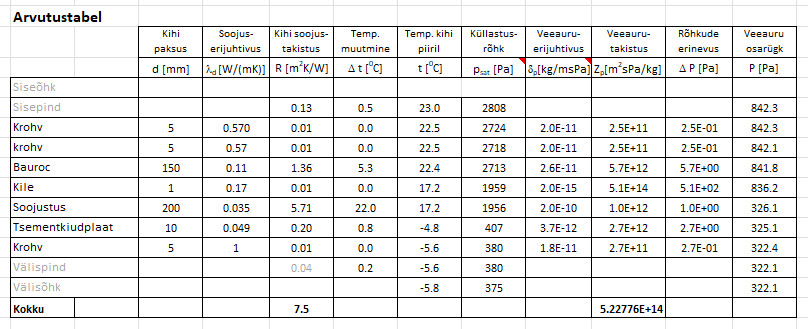
\includegraphics[width=.8\textwidth]{figures/01_analogues/04_calc_table.png}
    \caption{\textit{Niiskustehnilise toimivuse analüüsi tabeli näide}}
    \label{fig:excel_table_sample}
\end{figure}

Lõppkokkuvõttes analüüsi tulemused esitatakse graafiliselt diagrammi kujul, mille peale on kantud konstruktsiooni 
kihid, temperatuuri, veeauru küllastusrõhu ja veeauru osarõhu jaotuse graafikud (näide on toodud pildil \ref{fig:excel_graph_sample}). 
Selle tegevuse eesmärk on hinnata kondenseerumise riski konstruktsiooni kihtides. Veeauru osa- ja küllastusrõhu 
suhe on suhteline niiskus, vastavalt mida lähedam osarõhu graafiku joon küllasturõhu joonele -- seda kõrgem on 
antud konstruktsiooni kohas suhteline niiskus. Juhul kui mingis punktis osarõhu joon saavutab küllastusrõhu 
joont -- tekib selles punktis kondensaat. 

\begin{figure}[ht]
    \centering
    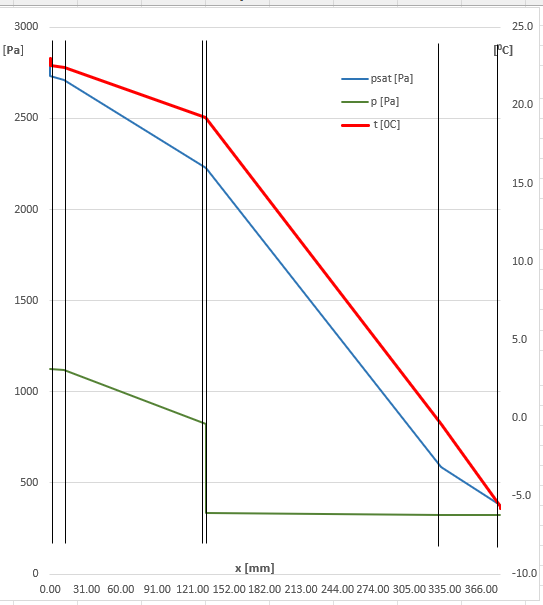
\includegraphics[width=.6\textwidth]{figures/01_analogues/05_excel_grafic_sample.png}
    \caption{\textit{Niiskustehnilise toimivuse analüüsi graafiku näide}}
    \label{fig:excel_graph_sample}
\end{figure}



\section{Olemasolevad lahendused ja turu analüüs}
Üks populaarsematest analoogidest, mida kasutatakse sealhulgas ka Eestis, on Saksa päritoluga tarkvara \textbf{Ubakus}. 
Tegemist on veebirakenduse kujul kommertstarkvaraga, mille \textit{demo}-versioon on saadaval tasuta (pilt \ref{fig:ubakus_sample}). 
\begin{figure}[ht]
    \centering
    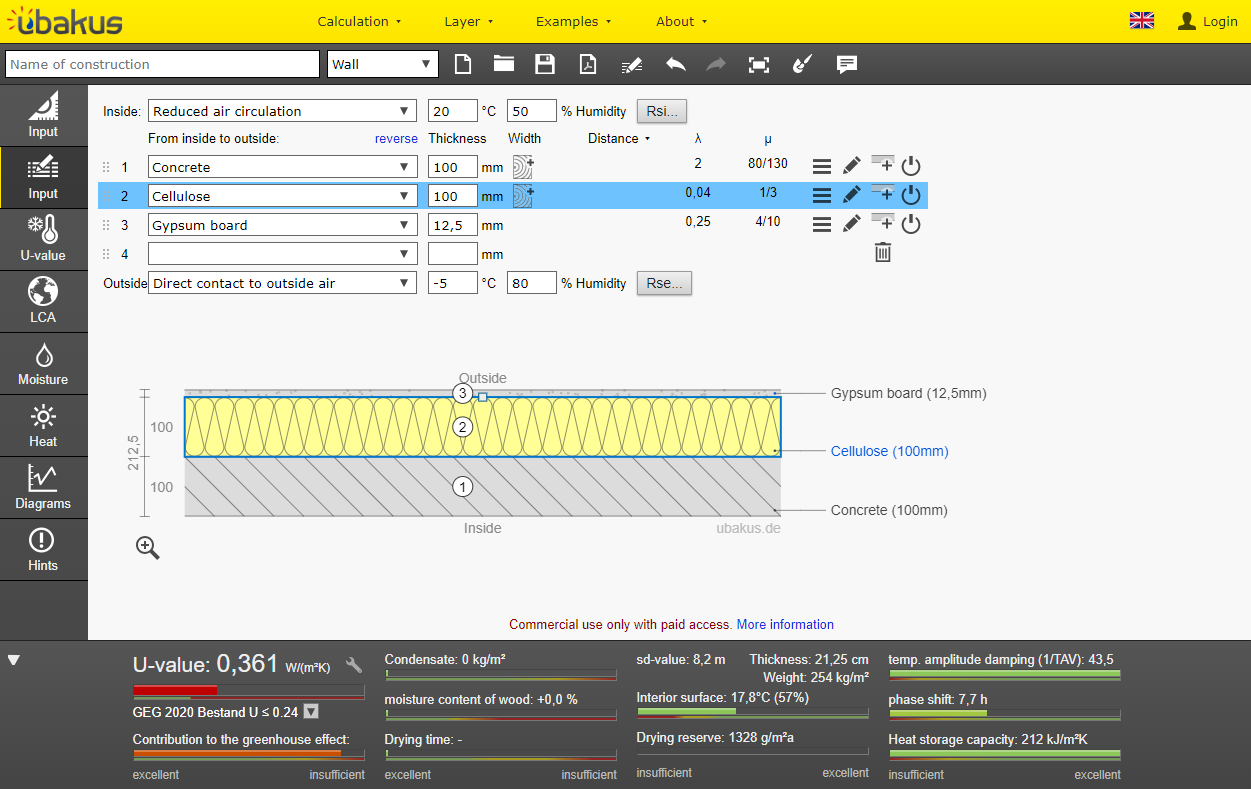
\includegraphics[width=.8\textwidth]{figures/01_analogues/01_ubakus.png}
    \caption{\textit{Ubakus veebirakenduse ekraanitõmmis.}}
    \label{fig:ubakus_sample}
\end{figure}

\textbf{Ubakus} võimaldab teostada konstruktsiooni niiskustehnilist analüüsi. Kasutajaliides võidaldab 
mudeldada mitmest kihist koosneva konstruktsiooni, valides igale kihile paksust ja materjali, millest 
kiht koosneb. Tugev eelis on see, et tarkvaraga saab analüüsida ka mittehomogeensete (mitemest erinevast 
materjalist, nt puitsõrestiksein) kihtidega konstruktsioone - pilt \ref{fig:ubakus_layers}

\begin{figure}[ht]
    \centering
    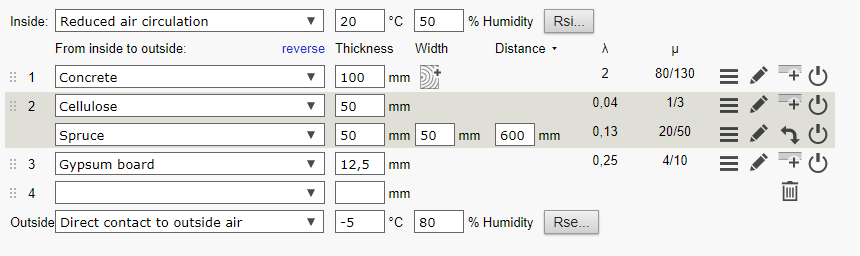
\includegraphics[width=.6\textwidth]{figures/01_analogues/02_ubakus_layers.png}
    \caption{\textit{Ubakus: konstruktsiooni kihtide lisamine.}}
    \label{fig:ubakus_layers}
\end{figure}

Ehitusmaterjalide valik, mida on võimalik konstruktsiooni mudeldamisel kasutada, on piisavalt lai 
(aga tasuta versioonis piiratud). Tasulises versioonis on samuti võimalik ka oma materjalide 
lisamine ja kasutamine. Puuduseks on see, et teatud osa baasis olevatest ehitusmaterjalidest on Saksamaal
turustatavad materjalid, mistõttu selle tarkvara kasutades Eestis peab kas sisestama kõik vajalikud 
materjalid käsitsi, või kasutada Saksa analoogid ning arvestada sellest tulenevaarvutuste ebatäpsusega.
\begin{figure}[ht]
    \centering
    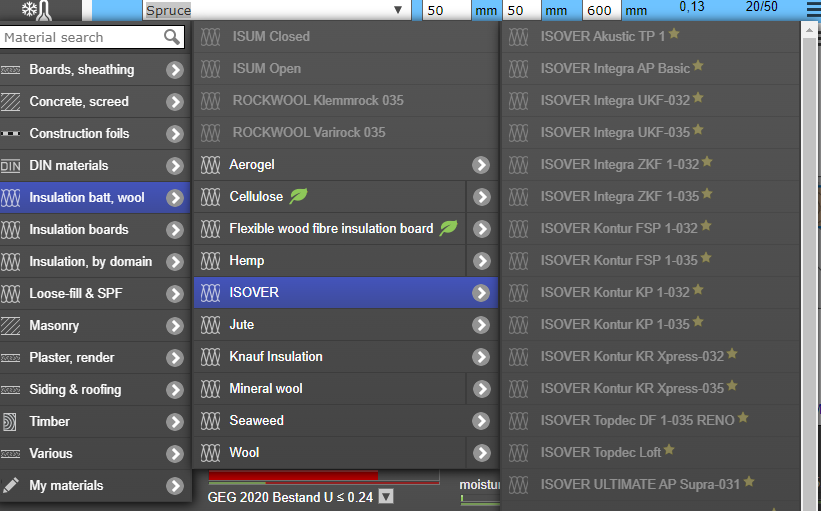
\includegraphics[width=.6\textwidth]{figures/01_analogues/03_ubakus_materials.png}
    \caption{\textit{Ubakus: ehitusmaterjalide valik baasis.}}
    \label{fig:ubakus_materials}
\end{figure}
